\documentclass{beamer}
	\usepackage[utf8]{inputenc}		% required for umlauts
	\usepackage[english]{babel}		% language
	%\usepackage[sfdefault]{roboto}	% enable sans serif font roboto
	%\usepackage{libertine}			% enable this on Windows to allow for microtype
	\usepackage[T1]{fontenc}		% required for output of umlauts in PDF

	\usepackage{mathtools}		% required for formulas

	\usepackage{caption}		% Customize caption aesthetics
	\usepackage{tcolorbox}		% fancy colored boxes
	\usepackage{xcolor}			% Highlighting
	\usepackage{soul}
	\usepackage{graphicx}		% required to insert images
	\usepackage[space]{grffile} % insert images baring a filename which contains spaces
	\usepackage{float}			% allow to forcefully set the location of an object

	\usepackage[tracking=true]{microtype} % required to change character spacing

	\usepackage[style=numeric,backend=biber]{biblatex}
	\usepackage{hyperref}		% insert clickable references

	\usepackage{datetime}		% flexible date specification
	\newcommand{\leadingzero}[1]{\ifnum#1<10 0\the#1\else\the#1\fi}
	\newcommand{\todayddmmyyyy}{\leadingzero{\day}.\leadingzero{\month}.\the\year}
	\newcommand{\mathcolorbox}[2]{\colorbox{#1}{$\displaystyle #2$}}

	\usepackage{geometry}
	\usepackage{scrextend}		% allow arbitrary indentation

	\usepackage{color}

	\addbibresource{../literature.bib}

	\setbeamercolor{title}{fg=orange}
	\setbeamertemplate{title}{
		\color{orange}
		\textbf{\inserttitle}
	}
	\setbeamercolor{tableofcontents}{fg=orange}
	\setbeamercolor{section in toc}{fg=black}
	\setbeamercolor{subsection in toc}{fg=black}
	\setbeamertemplate{frametitle}{
		%\vspace{0.5em}
		\color{orange}
		\begin{center}
			\textbf{\insertframetitle} \\
			{\small \insertframesubtitle}
		\end{center}
	}
	\setbeamertemplate{itemize item}{\color{black}$\bullet$}
	\setbeamertemplate{itemize subitem}{\color{black}$\circ$}
	\setbeamercolor{block title}{fg=black}
	\captionsetup{font=scriptsize,labelfont={bf,scriptsize}}

	\title{Optimization of Particle Identification}
	\subtitle{The Analysis Software behind Particle Discoveries}
	\author[Edenhofer]{Gordian Edenhofer}
	\institute[LMU]{
	Working Group of Prof.~Dr.~Kuhr \\
	Faculty of Physics \\
	University of Munich
	}
	\date[PSRC 2018]{Physics Student Research Conference, 09. June 2018}
	\subject{Particle Physics}


\begin{document}

\begin{frame}
	\titlepage
\end{frame}

\begin{frame}
	\frametitle{Agenda}

	\begin{columns}[T]
		\begin{column}{.6\textwidth}
			\vspace{3.5em}
			\tableofcontents[hideallsubsections]
		\end{column}
		\begin{column}{.39\textwidth}
			\begin{figure}
				\centering
				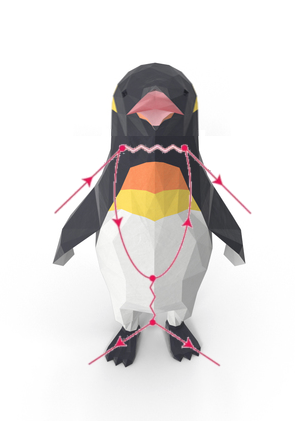
\includegraphics[width=\textwidth,height=\textheight,keepaspectratio]{{{../res/Awesome Penguin Diagram}}}
				\caption{Penguin Diagram in front of a Low-Poly Penguin. Patchwork.}
			\end{figure}
		\end{column}
	\end{columns}
\end{frame}

\section[Belle 2]{Belle 2 Experiment}
\begin{frame}
	\frametitle{\insertsection}

	\begin{columns}[T]
		\begin{column}{.6\textwidth}
			\vspace{3em}
			\begin{itemize}
				\item Standard Model Validation
				\item Electron-, Positron-Accelerator
				\item $B$-Meson fabric
			\end{itemize}
			\begin{itemize}
				\item Cross section: $~10 \mathrm{\mu m} \times 60 \mathrm{nm}$
				\item Asymmetric beams at $\sqrt{S} = 10.58 \mathrm{GeV}$
				\item High Luminosity
			\end{itemize}
		\end{column}
		\begin{column}{.4\textwidth}
			\begin{figure}
				\centering
				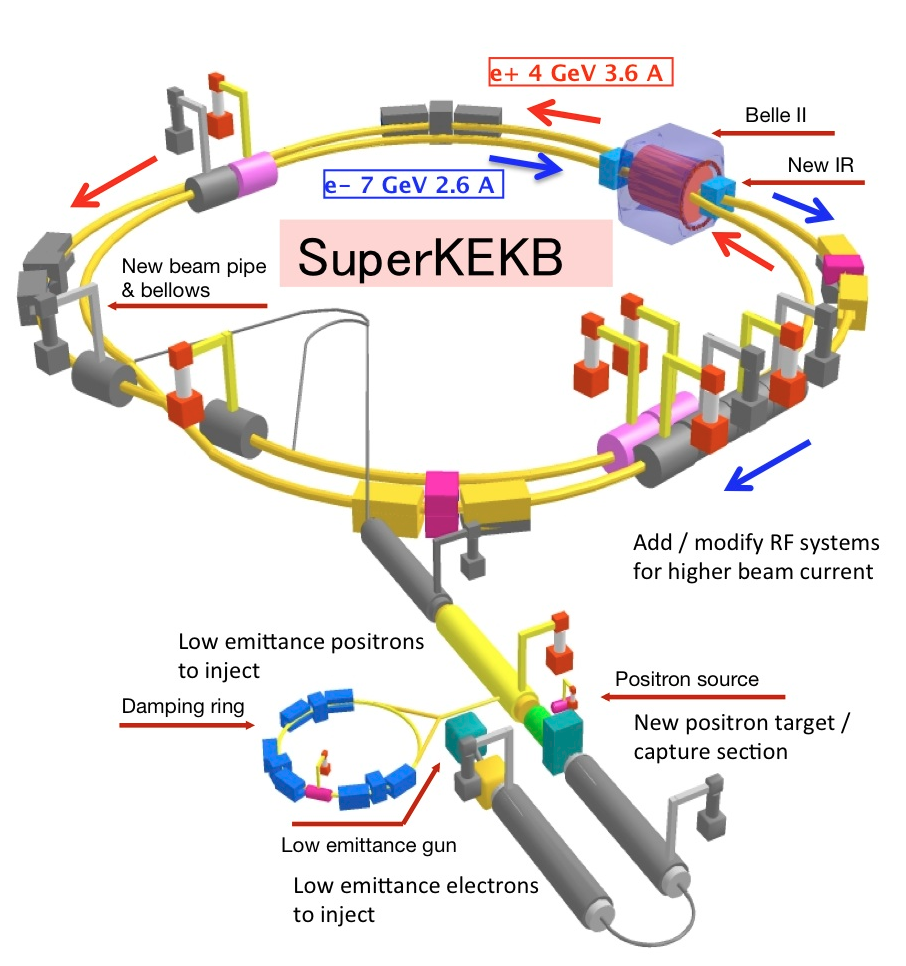
\includegraphics[width=\textwidth,height=0.8\textheight,keepaspectratio]{{{../res/Belle 2 accelerator: SuperKEKB}}}
				\caption{Sketch of the Belle 2 accelerator SuperKEKB. Adapted from \cite{Belle2Collaboration:SuperKEKBSketch}.}
			\end{figure}
		\end{column}
	\end{columns}
\end{frame}

\subsection{Detector Systems}
\begin{frame}
	\frametitle{\insertsection}
	\framesubtitle{\insertsubsection}

	\begin{columns}[T]
		\begin{column}{.6\textwidth}
			\vspace{1.5em}
			\begin{itemize}
				\item \textbf{P}i\textbf{X}el \textbf{D}etector
				\item \textbf{S}ilicon \textbf{V}ertex \textbf{D}etector
				\item \textbf{C}entral \textbf{D}rift \textbf{C}hamber
				\item \textbf{T}ime \textbf{O}f \textbf{P}ropagation counter
				\item \textbf{A}erogel \textbf{RICH} counter
				\item \textbf{E}lectromagnetic \textbf{C}a\textbf{L}orimeter
				\item $\boldsymbol{K}^0_{\boldsymbol{L}}$/$\boldsymbol{\mu}$ detector
			\end{itemize}
		\end{column}
		\begin{column}{.4\textwidth}
			\begin{figure}
				\centering
				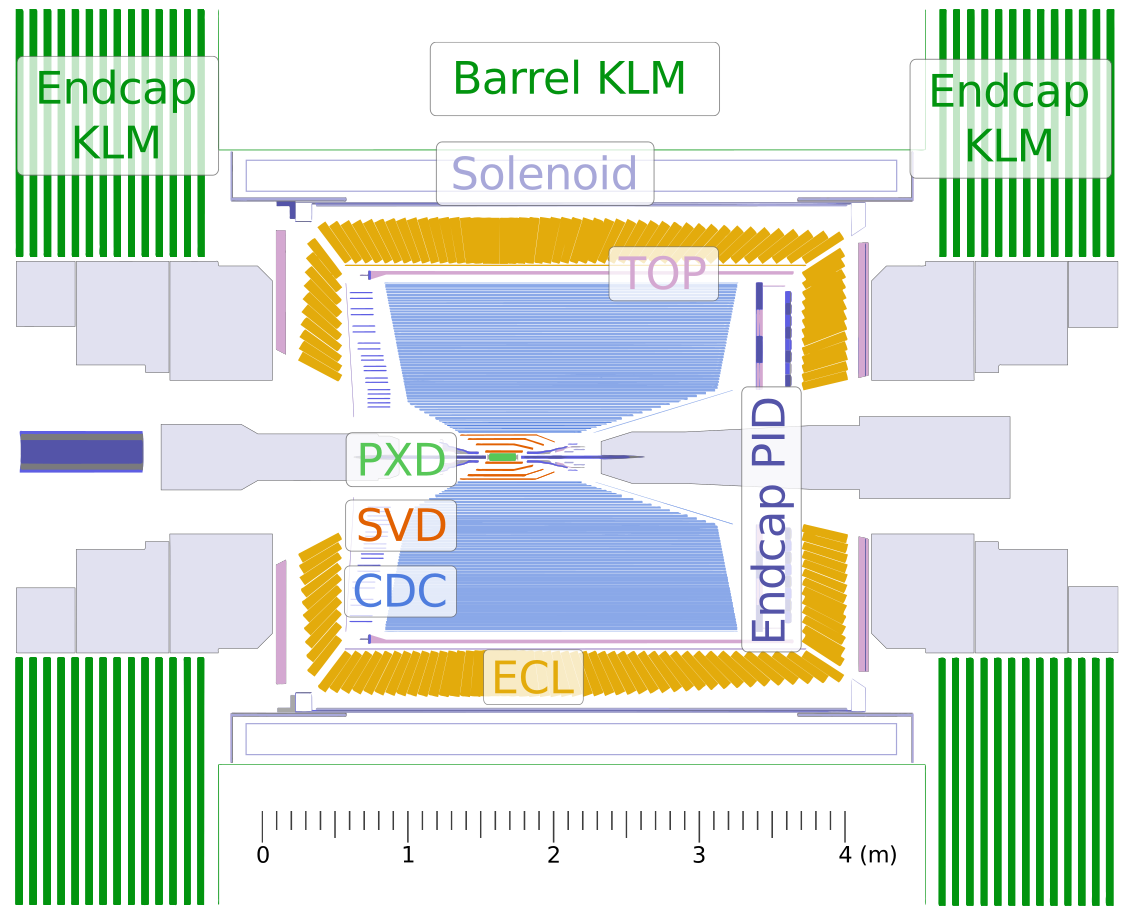
\includegraphics[width=\textwidth,height=0.5\textheight,keepaspectratio]{{{../res/Belle 2 detector systems}}}
				\caption{Belle 2 detector components. Taken from \cite{Pulvermacher:SuperKEKBDetectorComponents}.}
			\end{figure}
		\end{column}
	\end{columns}
\end{frame}


\section[Statistics]{Statistics for Particle Analysis}
\subsection{Bayes' Theorem}
\begin{frame}
	\frametitle{\insertsection}
	\framesubtitle{\insertsubsection}

	\begin{alertblock}{Bayes' Theorem}
		\centering
		$\mathcolorbox{yellow}{P(A|B) = \frac{P(B|A) \cdot P(A)}{P(B)}}$
	\end{alertblock}
	\vspace{1em}

	The likelihood of a particle may vary depending on its
	\begin{itemize}
		\item abundance
		\item detector yields (angle between particle and beam; transverse momentum)
		\item point of detection
	\end{itemize}
\end{frame}

\subsection{Bayesian Approach}
\begin{frame}
	\frametitle{\insertsection}
	\framesubtitle{\insertsubsection}

	\textbf{Univariate:} \\
	Probability dependant on one detector variable, e.g. $P(\pi|p_t)$ \\

	\vspace{2em}

	\textbf{Multivariate:} \\
	Probability dependant on a multitude of detector variable, e.g. $P(\pi|p_t, \Theta)$
\end{frame}

\subsection{Receiving Operating Characteristic}
\begin{frame}
	\frametitle{\insertsection}
	\framesubtitle{\insertsubsection}

	Goodness of a selection via \\
	True Positive Rate / False Positive Rate

	\begin{figure}
		\centering
		\includegraphics[width=\textwidth,height=0.6\textheight,keepaspectratio]{{{../res/Sample Receiver Operating Characteristic (ROC) curve}}}
		\caption{Sample Receiver Operating Characteristic (ROC) curve.}
	\end{figure}
\end{frame}

\section{Particle Identification}
\subsection{Existing Methods}
\begin{frame}
	\frametitle{\insertsection}
	\framesubtitle{\insertsubsection}

	\begin{columns}
		\begin{column}{0.47\textwidth}
			\begin{table}
				\begin{tabular}{l|l}
					pionID & $\mathcal{L}_{\pi} / (\mathcolorbox{yellow}{\mathcal{L}_{\pi}} + \mathcal{L}_{K})$ \\
					kaonID & $\mathcal{L}_{K} / (\mathcal{L}_{K} +\mathcolorbox{yellow}{\mathcal{L}_{\pi}})$ \\
					protonID & $\mathcal{L}_{p} / (\mathcal{L}_{p} +\mathcolorbox{yellow}{\mathcal{L}_{\pi}})$ \\
					electronID & $\mathcal{L}_{e} / (\mathcal{L}_{e} +\mathcolorbox{yellow}{\mathcal{L}_{\pi}})$ \\
					muonID & $\mathcal{L}_{\mu} / (\mathcal{L}_{\mu} +\mathcolorbox{yellow}{\mathcal{L}_{\pi}})$ \\
					deuteronID & $\mathcal{L}_{d} / (\mathcal{L}_{d} +\mathcolorbox{yellow}{\mathcal{L}_{\pi}})$
				\end{tabular}
				\caption{ParticleID detector variables for selection and further analysis.}
			\end{table}
		\end{column}
		\begin{column}{0.5\textwidth}
			\begin{table}
				\begin{tabular}{l|l}
					pidProbabilityPion & $\mathcal{L}_{\pi} / \mathcal{L}_{all}$ \\
					pidProbabilityKaon & $\mathcal{L}_{K} / \mathcal{L}_{all}$ \\
					pidProbabilityProton & $\mathcal{L}_{p} / \mathcal{L}_{all}$ \\
					pidProbabilityElectron & $\mathcal{L}_{e} / \mathcal{L}_{all}$ \\
					pidProbabilityMuon & $\mathcal{L}_{\mu} / \mathcal{L}_{all}$ \\
					pidProbabilityDeuteron & $\mathcal{L}_{d} / \mathcal{L}_{all}$ \\
					\hline
					\multicolumn{2}{c}{$\mathcal{L}_{all} = \sum \limits_{x \in {\pi, K, p, e, \mu, d}} \mathcal{L}_{x}$}
				\end{tabular}
				\caption{Likelihood-Ratios for particle selection and further analysis.}
			\end{table}
		\end{column}
	\end{columns}
\end{frame}

\section{Identification Rate Comparisons}
\subsection{Particle Distributions}
\begin{frame}
	\frametitle{\insertsection}
	\framesubtitle{\insertsubsection}

	\begin{figure}
		\centering
		\includegraphics[width=\textwidth,height=0.6\textheight,keepaspectratio]{{{../res/charged 01/General Purpose Statistics: True Particle Abundances in the K+-Data}}}
		\caption{True particle abundance in the simulated data.}
	\end{figure}
\end{frame}

\subsection{ROC \& PPV}
\begin{frame}
	\frametitle{\insertsection}
	\framesubtitle{\insertsubsection}

	\begin{figure}
		\centering
		\includegraphics[width=\textwidth,height=0.6\textheight,keepaspectratio]{{{../res/charged 01/Diff Statistics: K Identification via PID, by pt & cos(Theta)}}}
		\caption{Kaon Identification via PID and Bayes by $p_t$ \& $\cos(\Theta)$.}
	\end{figure}
\end{frame}

\begin{frame}
	\frametitle{\insertsection}
	\framesubtitle{\insertsubsection}

	\begin{figure}
		\centering
		\includegraphics[width=\textwidth,height=0.6\textheight,keepaspectratio]{{{../res/charged 01/Diff Statistics: K Identification via PID, via flat Bayes}}}
		\caption{Kaon Identification via PID and via flat Bayes (pidProbability).}
	\end{figure}
\end{frame}

\subsection{Confusion Matrix}
\begin{frame}
	\frametitle{\insertsection}
	\framesubtitle{\insertsubsection}

	\begin{figure}
		\centering
		\includegraphics[width=\textwidth,height=0.6\textheight,keepaspectratio]{{{../res/charged 01/Diff Heatmap: Heatmap of epsilonPID Matrix for an exclusive Cut via PID, by pt & cos(Theta)}}}
		\caption{Heatmaps of row-wised normed confusion matrix for an exclusive Cut via PID and Bayes by $p_t$ \& $\cos(\Theta)$ showing the particle identification and confusion rates.}
	\end{figure}
\end{frame}

\subsection{Conclusion}
\begin{frame}
	\frametitle{\insertsection}
	\framesubtitle{\insertsubsection}

	\textbf{Current work:}\\
	\begin{itemize}
		\item Noticeable improvements using multivariate Bayesian approach
		\begin{itemize}
			\item Slight losses for certain False Positive Rates
			\item Slight down-turns for certain False Positive Rates
		\end{itemize}
		\item Increased flexibility due to honoring decay-specific abundances
	\end{itemize}

	\vspace{2em}
	\textbf{Work in Progress \textit{(feel free to ask me about it)}:}\\
	\begin{itemize}
		\item Machine Learning
	\end{itemize}
\end{frame}

\section*{Bibliography}
\begin{frame}
	\frametitle{\insertsection}

	\printbibliography
\end{frame}

\section{Appendix}
\subsection{Terminology}
\begin{frame}
	\frametitle{\insertsection}
	\framesubtitle{\insertsubsection}

	\begin{columns}
		\begin{column}{0.47\textwidth}
			\begin{block}{\textbf{T}rue \textbf{P}ositive \textbf{R}ate (TPR)}
				Elements which are correctly identified as being correct
			\end{block}
			\begin{block}{\textbf{T}rue \textbf{N}egative \textbf{R}ate (TNR)}
				Elements which are correctly identified as being incorrect
			\end{block}
		\end{column}
		\begin{column}{0.5\textwidth}
			\begin{block}{\textbf{F}alse \textbf{P}ositive \textbf{R}ate (FPR)}
				Elements which are incorrectly identified as being correct
			\end{block}
			\begin{block}{\textbf{F}alse \textbf{N}egative \textbf{R}ate (FNR)}
				Elements which are incorrectly identified as being incorrect
			\end{block}
		\end{column}
	\end{columns}
	\vspace{2em}
	\mathcolorbox{yellow}{
		\begin{tabular}{l|ll}
			Veracity & True = correct & False = incorrect \\
			Identification & Positive = accepted & Negative = rejected
		\end{tabular}
	}
\end{frame}

\end{document}
